\documentclass[12pt]{article}

\usepackage{sbc-template}
\usepackage{graphicx, url}
\usepackage{hyperref}
\usepackage[utf8]{inputenc}
\usepackage[rightcaption]{sidecap}

\graphicspath{ {./images/} }
     
\sloppy

\title{Video-based parking spot detection using machine learning}

\author{Olga Turcan, Viorel Gurdis, Raul-Robert Zavaczki}

\address{Babes-Bolyai University, Cluj-Napoca}


\begin{document} 

\maketitle

\begin{abstract}
  Living in a big city, it's a common problem to find available parking 
  spaces for your car. Having a real time parking space 
  detection system based on images provided by CCTVs could considerably 
  improve the parking experience at a relatively low cost.
\end{abstract}

\section{Introduction}

Statistically the average time spent searching for a parking spot represents \textbf{7.8 minutes}.
That is a waste of time and can also cause traffic congestion. There are several types of 
parking spaces monitoring systems, including counter-based and sensor-based, which try to solve the mentioned problem.
Counter-based systems work by counting cars at the parking lot entrance, but their disadvantage is that they don't provide 
concrete informations about available spots, leaving the task of finding the place to the driver.
A more precise solution could be sensor-based systems which provide availability information about each 
spot specifically. However, this solution implies higher costs (c.a \textbf{\$40} per unit). 
An alternative approach would be using video provided by already installed surveillance cameras for real-time 
detection by implementing a computer vision system.
This method relies on the detection of vehicles in delimited space areas and classification of a spot as 
available or occupied. The processed information will be delivered by a server in form of a web page and updated 
in real-time, which would make the solution accessible for everyone. That would definetely save time of the driver 
and considerably reduce traffic problems.
Challenges that we should expect will be related to the scalability of the application. We should, for example, take into 
consideration that the application should work in different weather conditions. We also focus on the accessibility 
of the processed information in real-time, for which we will try to compare different AI algorithms and will choose 
the one with the best balance between accurate results and small processing time.

\section{Related Work}

One approach to video-based real-time parking space detection application 
was described in the academic paper of \cite{tschentscher}. To minimize 
weather and lighting conditions influences and to maximize the accuracy of the 
results, the approach evaluates several combinations of feature extractors and 
machine learning algorithms. They used a self-built dataset containing 
ca. 10,000 samples, from which they extracted features like 
Color Histograms [RGB, HSV, YUV] (to distinguish between asphalt color and the 
cars, to solve problems with brightness), Gradient Histograms, 
Difference-of-Gaussian Histograms and Haar-like (to extract edge information). 
Three classifiers were trained and compared to each other based on features 
mentioned above: k-Nearest Neighbor, Linear Discriminant Analysis, Support 
Vector Machine. The final solution relies on HSV color histogram and 
Difference-of-Gaussian features and a SVM classifier, which reached an 
accuracy of 99.8\%.
\par
An alternate approach for vacant parking space detection is described in 
\cite{debaditya}, which uses features extracted by a pre-trained CNN to 
train an SVM classifier for the detection of parking occupancy in a 
CCTV image sequence.
The CNN extracts features from the publicly available PKLot dataset which 
consists of more than 12,000 images collected from 3 parking sites on 
different weather conditions. 
Consequently, the extracted features from images of the PKLot dataset 
were used to train and test a binary SVM classifier.
The evaluation of the classification accuracy is done by cross validation 
on the PKLot dataset and the transfer learning ability on the Barry 
Street dataset, which was created for the purpose of that research and 
includes a sequence of images captured by a camera overlooking a street 
with marked parking places.
\par
The binary classification using the deep features achieved consistently 
reliable results with an average accuracy of 99.7\% across different weather 
conditions for the PKLot dataset.
As transfer learning was a more challenging task because the classifier 
was required to recognize unfamiliar images, the classification of Barry 
Street images achieved the overall accuracy of 96.65\%.
It is worth mentioning that the processing time for each image region 
representing a parking space is 0.067 seconds on a simple desktop computer 
which means it takes approximately 2 seconds to process all the parking 
spaces in an image and hence the solution is suitable for real-time 
applications without any dedicated hardware.
\par
A more rudimentary approach for parking spots detection was used in \cite{roman},
but they provided valuable information on the different approaches used
to determine whether a parking spot is free or not. Also the FMPH dataset
was introduced, consisting of 1,093 pictures depicting 25,139 parking
spots during a 30-day timespan, taken in various weather conditions.
For detecting the parking spots in an image, they provided an API that
allowed an administrator to manually draw masks of each parking spot.
Assuming that the camera rotation doesn't change, they mapped the masks
for each subsequent image, allowing them to generate an 80x80 pixel
image for each parking spot in an image, allowing them to normalize
the inputs.
\par
The most notably performer was an MLP(15,15) classifier, which got an accuracity
of 88.2\% on the mentioned FMPH dataset. Among the other tested approaches
were kNN algorithms with k=1 and k=3, getting an accuracity of 82.2\% and
82.3\% respectively. Another approach discussed in the paper is using
Logistic Regression to classify whether a parking spot is free or not,
but it proved to be the most underperforming algorithm used, scoring
only 74,7\% accuracity.

\subsection{Useful Tools}

The following tools were used for implementing above mentioned approaches.
\begin{itemize}
  \item Tensorflow
  \item Keras
  \item scikit-learn
\end{itemize}

\section{Methodology}
Our research focuses on detecting the occupancy of parking lots from the images obtained by CCTVs.
The algorithm we've implemented consists of a Convolutional Neural Network which was trained on the opensource 
\cite{cnrpark} dataset which consists of 150x150 pixels patches grouped into 2 categories: busy and free.
Our Keras model with Tensorflow backend has the following architecture: One convolutional layer having 3x3 image kernels,
followed by a max-pooling layer with 2x2 pool size, a flatten layer, which reshapes the tensor for the upcoming dense layer 
with ReLU as activation. To complete our CNN, we need to give it the ability to actually make predictions. 
We’ll do that by using the standard final layer for a multiclass classification problem: 
the Softmax layer, a fully-connected (dense) layer that uses the Softmax function as its activation.
Before begining the training, we added some configurations during the compilation step:
As \textbf{optimizer}, we decided for the Adam gradient-based optimizer and for the \textbf{loss function} 
we used the sparse-categorical cross-entropy loss.

\begin{SCfigure}[0.5][h]
\caption{Example of 150x150 px patches, free and occupied}
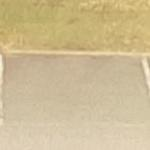
\includegraphics[width=0.2\textwidth]{20150703_0810_10}
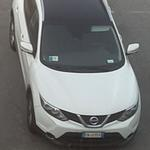
\includegraphics[width=0.2\textwidth]{20150703_0810_45}
\label{fig:resultimg}
\end{SCfigure}


\subsection{Experimental Design}
In order to detect available lots in a parking, our application "ParkinGo" uses a Machine Learning approach.
Each lot is initially marked manually and stored into a database. By uploading the image of the entire parking area,
our algorithm is able to iterate through all labeled regions of interest (ROIs), scale each ROI from original image to the coresponding resolution 
and then apply Convolutional Neural Network, that is able to predict with 99\% accuracy, which lot is occupied and which one is empty.
The average percentage of correctly classified parking spots from an input image is 96\%, as seen in the figure \ref{fig:resultimg}.

\begin{SCfigure}[0.5][h]
\caption{Obtained image after labeling the ROIs}
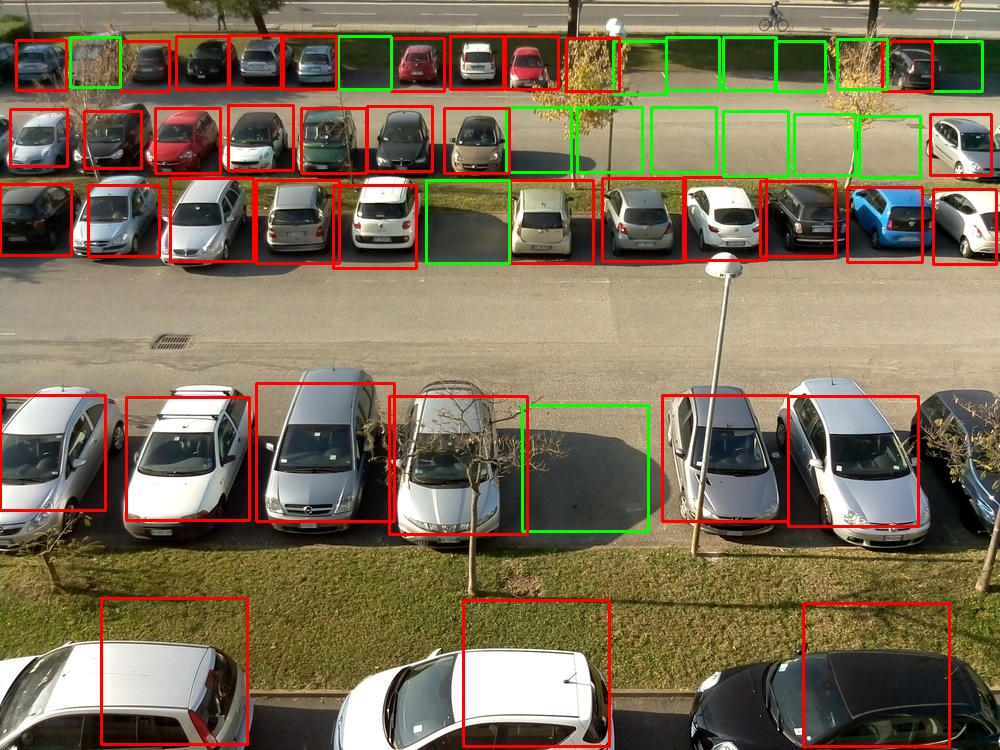
\includegraphics[width=0.6\textwidth]{2015-11-12_0947}
\label{fig:resultimg}
\end{SCfigure}

\bibliographystyle{sbc}
\bibliography{sbc-template}

\end{document}
